%FB comment from design section comparison: Please bring back the followinf: "The bracketed prediction reference: "recent findings show that modern machine learning models achieve comparable accuracy to humans when predicting BMI from such images" — the substantive claim that models can match humans on facial-feature → body-weight prediction, with [evidence] placeholder. Cut entirely from the new text. The author may want to bring this back if a referee asks how plausible the equal-performance framing is."
%FB comment from design section comparison: Please make sure that this point is made somewhere in this section: "The aside: "to enhance the clarity and intuitiveness of the task for participants, we chose to use weight rather than BMI as the prediction target" — a small design-choice justification. Currently absent from the new design section."
\section{Experimental Design} \label{design}

We conducted a preregistered online experiment on the British platform Prolific between February and June 2023, recruiting $322$ participants from the United Kingdom. The design combines a between-subject manipulation of whether costly punishment is possible with a within-subject elicitation of conditional punishment behaviour.

Within each condition, participants assumed one of two roles. Player~A decides whether to make a payoff-relevant prediction for Player~B directly, or to delegate the prediction to an algorithm calibrated to perform as well as she does. Player~B is the third party whose payoff depends on the outcome of Player~A's prediction; in the \textit{Punishment} condition Player~B may subsequently punish Player~A, conditional on both the delegation decision and the realised outcome, while in the \textit{No-Punishment} condition no punishment is possible. Figure~\ref{fig:treatments} summarises the basic structure.
%FB comment: Is it justified to call Player B a third party? On the one hand, there are only two roles, so calling B a third party may be weird, but on the other hand, B is fully dependent on A. 

\begin{figure}[!htbp]
    \centering
    \footnotesize
    \caption{Conditions overview}

    \scalebox{0.9}{
    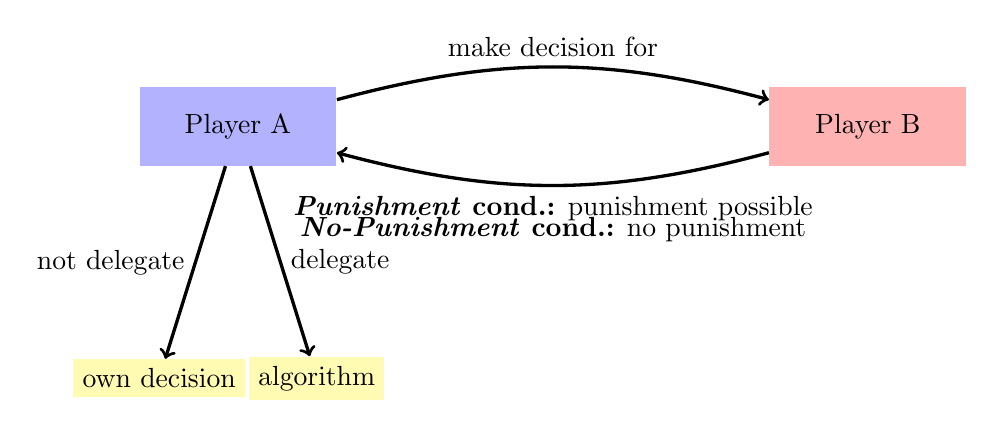
\begin{tikzpicture}[scale=1, every node/.style={scale=1}]
            %boxes
            \node (A) at (1,-3.2) [fill=yellow!30] {algorithm};
            \node (OD) at (-1,-3.2) [fill=yellow!30] {own decision};
            \node (D) at (0,0) [fill=blue!30, minimum width=2.5cm, minimum height=1cm] {Player A};
            \node (E) at (8,0) [fill=red!30, minimum width=2.5cm, minimum height=1cm] {Player B};

            %arrows
            \draw[<-, very thick] (A) to node[right] {delegate} (D);
            \draw[<-, very thick] (OD) to node[left] {not delegate} (D);
            \draw[->, very thick, bend left = 15] (D) to node[above] {make decision for} (E);
            \draw[<-, very thick, bend right = 15] (D) to node[below, align=center] {\textbf{\textit{Punishment} cond.:} punishment possible\\[-1ex]\textbf{\textit{No-Punishment} cond.:} no punishment} (E);

    \end{tikzpicture}
    }
    \label{fig:treatments}
\end{figure}

\subsection*{Sample}

We targeted a balanced design of 80~participants per role per condition, for a planned sample of 320~subjects. The cell size was set to detect, at conventional power, the effects anticipated from the responsibility-avoidance literature; the underlying ex-ante power calculation is reproduced in Appendix~\ref{appendix:pap}. Attrition and subsequent re-matching brought the realised sample to 322 participants ($161$ Player~A and $161$ Player~B), with a CONSORT-style flow diagram broken down by condition and role in Appendix~\ref{appendix:attrition}.
%FB comment: The statement is not backed by evidence. We should say something like: With this sample size, at conventional power, one can detect a treatment effect of X given standard deviation of Y [Perhps do the following calculations and show a figure in the appendix: At 80% power with the given sample size and alpha=0.05, plot the treatment effect size and standard deviation in % of the treatment effect size on the y and x axis or x and y axis]. 
%FB comment: Let's only refer to the CONSORT-style flow diagram at the end of talking about the procedure for player A and player B. Also, let's not call it CONSORT style diagram, let's just stay generic and say that the details of the experimental timeline/procedure can be understood from figure X in the appendix.

The experiment was programmed in oTree~\citep{chen_otree_2016} and run via Prolific. Eligibility followed Prolific's standard quality screens---minimum 95\% prior approval rate, no warnings on file, fluent-English filter, and UK residence---together with a desktop-only restriction (no mobile or tablet) to keep the screen layout consistent across subjects. Player~A spent on average 12~minutes on the study and earned an average bonus of $\pounds 2.49$ on top of the Prolific show-up fee; Player~B spent on average 8~minutes and earned an average bonus of $\pounds 2.30$.\footnote{Bonus computed deterministically from cleaned data per the experimental rules: random-round task payoff (expectation over the uniform draw), belief-about-own-score payoff ($\pounds 0.30$ times the mass placed on the realised score), belief-about-distribution payoff (expectation over the uniform random draw of which score is checked), and---for Player~A in the \textit{Punishment} condition---expected punishment from the matched Player~B's strategy-method choice in the realised cell, with $\pounds 0.10$ per cell of strategy-method punishment cost for Player~B. The bonus excludes the risk-elicitation MPL payoff (raw-data column not retained in the cleaned files); including it would add roughly $\pounds 0.30$--$\pounds 0.50$ per subject.}
%FB comment: The whole "Sample" subsection seems to overlap a lot with the "Sample, Attention and Balance" subsection in the results section. Please avoid repetition and please think about it and recommend where to include this information. It would also be possible to include some info in the design section and some in the results section. Let's discuss a plan first.

\subsection*{Procedure}

\subsubsection*{Player A}

After providing informed consent, Player~A completed ten incentivised rounds of a visual prediction task. In each round, she predicted a person's weight from a facial image and the person's height. Predictions could be entered via slider or typed directly in kilograms, pounds, or stones-and-pounds; no feedback was provided between rounds.\footnote{All individuals depicted in the images had explicitly consented to the use of their photographs for research purposes.} At the end of the experiment, one of the ten rounds was randomly selected for payment: Player~A earned $\pounds 4$ if her prediction in that round was within $10$~lbs of the true weight and $\pounds 2$ otherwise. These initial rounds served three purposes simultaneously: they established a stake from which any later punishment could be deducted; they familiarised Player~A with the task; and they generated the performance data needed to calibrate the algorithm.

The choice of a visual prediction task is deliberate. Algorithm preferences depend sensitively on the algorithm's perceived relative competence~\citep{dietvorst_algorithm_2015,logg_algorithm_2019}; as described below, our design neutralises this concern by calibrating the algorithm to match each subject's individual performance. The visual nature of the task makes algorithmic error plausible and lends credibility to the equal-performance claim, in contrast to purely mathematical tasks where subjects may be sceptical that an algorithm could ever fail~\citep{gogoll_rage_2018}. Predicting body weight from a facial image has been used in earlier experiments~\citep{logg_algorithm_2019} and arguably levels the playing field between human and algorithm: humans have a lifetime of practice at this mapping, while algorithms cannot easily exploit large training corpora here. Finally, we chose a prediction task involving genuine uncertainty rather than a setting with an obvious self-serving motive (as in classic dictator-game variations). This reflects the nature of many real-world applications of algorithms---financial forecasting, medical diagnosis, fraud detection---in which outcomes are inherently uncertain and performance is evaluated ex post.
%FB comment: Add a comment to the provided references here, because I will want to check whether this is precisely what these papers are about. Please do a first check yourself by reading through these papers.

After the ten rounds, Player~A was randomly paired with another participant, Player~B. Player~A was informed that her final, eleventh prediction would not affect her own payoff but would almost entirely determine the payoff of Player~B, who had not completed the prediction task himself: if the prediction fell within 10~lbs of the true weight, Player~B would receive a high payoff ($\pounds 5$); otherwise a low payoff ($\pounds 1$). Player~A then learned that she could either make the prediction herself or delegate it to an algorithm calibrated to mimic her own performance from the first ten rounds, so that on expectation the algorithm would produce the high payoff for Player~B at the same rate as Player~A would.
%FB comment: I would not say that Player A knew that the algorithm would mimic their own success chance. I would say something more neutral, such as "were told that the algithm performed equally well in the first 10 rounds." Also, it is not necessarily true, that even in expectation the algirthm would perform the same as Player A, because Player A could now put more effort. Please rephrase this or leave out this claim.

Concretely, the algorithm draws a Bernoulli outcome with success probability equal to Player~A's empirical accuracy rate over her first ten rounds. A subject who scored 3/10 in the initial rounds thus delegates to an algorithm that produces the high payoff for Player~B with $30\%$ probability. This individual-level Bernoulli calibration is the central design innovation relative to the closest precedent~\citep{feier_hiding_2022}, and it does substantive work in the identification argument. First, it makes the equal-performance claim literally true on average for every subject. Second, it strips any signal value that the delegation decision might otherwise carry about Player~A's beliefs concerning her own ability relative to the algorithm: a Player~B observing the delegation decision has no basis on which to read it as overconfident, lazy, or selfish. This closes off the most plausible third-party signal-extraction channel through which delegation might otherwise insulate the principal from punishment.
%FB comment: It "makes it literally true" for the first 10 rounds, but not necessarily for the last round, right?

The contrast with session-level calibration is consequential. Had the algorithm instead been calibrated to reflect aggregate performance across a pool of participants---as in \citet{feier_hiding_2022}---the delegation choice would be confounded by each subject's beliefs about her own ability relative to the pool. Indeed, \citet{feier_hiding_2022} report that the delegation decision in their setting is largely driven by perceived own performance relative to the algorithm. Pairing the algorithm to each subject individually, and making this common knowledge between Player~A and Player~B, strips this confound out by construction.

In the \textit{Punishment} condition, Player~A was further informed that Player~B could reduce her payoff by up to $\pounds 2$, with the deduction depending on both her delegation decision and the realised outcome. In the \textit{No-Punishment} condition, Player~B had no punishment option. The two delegation options (own decision / algorithm) were presented in random order across subjects, to control for any framing effect of which option appeared first. We attached no monetary cost to delegation: had we done so, no-delegation would have been the rational choice in the \textit{No-Punishment} condition by construction, masking any treatment effect on intrinsic preference. If Player~A chose not to delegate she was asked to make the final prediction and to state her confidence in having earned the high payoff for Player~B; this step was skipped if the algorithm made the prediction.
%FB comment: Here I am worried that the justification for the costlessness of delegation is not strong enough. I would perhaps add that making it costless gets us closer to the intrinstic preference without punishment (but not claim that it is weakly dominant to not delegate...because we do not know which other mechnaisms are at play) and, if true, say that this is standard in the literature.; The last sentence is arbitrary, because the second to last sentence already qualifies the condition under which the confidence was elicited. Let's drop the last sentence.

We then asked Player A to report her beliefs about Player B's punishment in each of the four scenarios resulting from the combination of delegation decision (yes/no) and prediction outcome (high/low payoff for Player B). Beliefs were elicited on the same scale as actual punishment ($\pounds 0$--$\pounds 2$ in $\pounds 0.10$ increments) and the four scenarios were presented in block-wise random order. We chose not to incentivise belief elicitation for three reasons. First, only two of the four scenarios remain payoff-relevant after the delegation decision, making the others purely hypothetical. Second, an incentivised mechanism could induce hedging behaviour. Third, an incentive-compatible scoring rule across four scenarios would have substantially increased task complexity. Because we are nonetheless interested in comparing punishment beliefs to actual punishment, we included an attention check on the belief-elicitation screen.\footnote{Subjects who failed the attention check are excluded from belief-related analyses, as preregistered.} In the \textit{No-Punishment} condition, no punishment was possible; we elicited beliefs about hypothetical punishment to maintain consistency across treatments.
%FB comment: Here I want to make a general comment: We have to think about how we talk about the pre-registration. Ideally, I would like to link it once in the beginning and then not refer to it, unless I deviate from the preregistration. I have put the pre-registration into a folder "pre-registration". Please read it and suggest all edits you would make to the draft based on it. The analysis should not change, we should only disclose if we deviate strongly from the pre-registration.

Player~A was then asked to assess her own performance in the first ten rounds by assigning a probability mass (summing to $100\%$) to each possible score from $0$ to $10$. This elicitation was incentivised: Player~A earned an additional $\pounds 0.30$ with the probability she had assigned to her actual score.\footnote{This mechanism is not incentive-compatible for risk-neutral participants. In practice only one subject assigned the full probability mass to a single score, suggesting that hedging considerations were modest.} She was also asked to estimate the population distribution of scores by assigning a share to each possible score from $0$ to $10$; one score was randomly drawn at the end of the experiment and Player~A earned $\pounds 0.30$ if her estimate for that score was within five percentage points of the realised population share.
%FB comment: The assessment of own performance will be influenced by already having received the information that the algorithm has performed the same. We should have probably elicited these performance related beliefs prior to the delegation decision, etc. Can you think of any reasons why it may still be a good idea to have done it afterwards, e.g. the delegation deciison is done, knowing that performance in the first 10 rounds was the same, so we are interested in the performance belief after having received that information. Perhaps to justify the elicitation of beliefs about others' performance, what could be a reason? To assess overconfidence/confidence relaive to others, but why? Regarding the footnote, I would not say that hedging motives were modest, because most people hedged in a sense by apportioning postivie probability mass for multiple options.

Finally, we elicited risk preferences using an incentivised multiple price list in the style of \citet{holt_risk_2002} and administered a short questionnaire on socio-demographic characteristics and technology affinity, before presenting Player~A with her preliminary payoff. Figure~\ref{fig:design_playerA} summarises the experimental timeline for Player~A.

\subsubsection*{Player B}

After providing informed consent, Player~B was told that he had been randomly matched with a Player~A and was introduced to the task Player~A had completed. He learned that his own payoff would be determined by the outcome of Player~A's eleventh prediction---$\pounds 5$ if it fell within 10~lbs of the true weight and $\pounds 1$ otherwise---while Player~A's payoff depended solely on her performance in the initial ten rounds. Crucially, Player~B was also told that Player~A could delegate the eleventh prediction to an algorithm calibrated to perform equally well as Player~A in the earlier rounds, and that Player~A herself was aware of this equal-performance calibration. The equal-performance claim is therefore common knowledge between the two players, a feature on which our identification argument rests.
%FB comment: I don't like "eleventh" prediction. Maybe "final", "additional", etc? 

In the \textit{Punishment} condition, Player~B could choose to reduce Player~A's payoff by up to $\pounds 2$ in $\pounds 0.10$ increments, at a personal cost of $\pounds 0.10$ per scenario in which positive punishment was chosen.\footnote{The cost is fixed per scenario rather than proportional to the punishment level, so that strictly positive punishment is always costly relative to no punishment but the cost does not increase with the severity of the sanction.} We elicited punishment decisions for all four combinations of delegation (yes/no) and outcome (high/low payoff for Player~B) via the strategy method, implementing only the decision matching the realised combination. The strategy method is essential to our power: a between-subject elicitation across cells would have required roughly four times the sample to detect cell-level differences at comparable power, well beyond our recruitment budget.\footnote{The strategy method may yield different absolute punishment levels than direct elicitation; we discuss the implications and a possible direct-method companion as future work in Section~\ref{conclusion}.} Because the punishment decision is the central outcome variable, we included an attention check on the punishment-elicitation screen.\footnote{The check asked the subject to confirm a numerical aspect of the payoff structure that had been displayed on the previous screen. Subjects failing this check are excluded from punishment-related analyses, as preregistered.} In the \textit{No-Punishment} condition, where actual punishment was not possible, we elicited hypothetical punishment decisions on the same scale to keep the experimental flow comparable across conditions. Player~B's perceptions of task difficulty, his risk preferences, and a short questionnaire followed, before he was presented with his final payoff. Figure~\ref{fig:design_playerB} summarises the experimental timeline for Player~B.
%FB comment: Can we say that the cost lied in foregoing an addition 0.10 pounds. I do not want the reader to think that the punishment was deducted. Also, please do not claim the we had a tight research budget or that the sample size would need to be four times higher. It's fine to keep a sentence that the strategy method gives us more power, but don't elaborate so much.

Once Player~B's decisions had been recorded, Player~A's final payoff was calculated and all participants were paid on the day of participation.

\subsection*{Hypotheses}

Our design tests two preregistered hypotheses, both grounded in the literature on responsibility avoidance through delegation~\citep{bartling_shifting_2012,coffman_intermediation_2011,oexl_shifting_2013,hamman_self-interest_2010,hill_does_2015,steffel_passing_2016} and on responsibility attributions to algorithmic decision-makers~\citep{feier_hiding_2022,kirchkamp_sharing_2019,gogoll_rage_2018}.

\begin{description}
\item[H1 (Delegation):] The introduction of potential punishment increases the likelihood that Player~A delegates the decision to the algorithm.
\item[H2 (Punishment):] Conditional on a low-payoff outcome for Player~B, Player~A is punished less when she delegated the decision to the algorithm than when she made it herself.
\end{description}

H1 is grounded in robust empirical evidence that responsibility avoidance shapes delegation decisions involving human intermediaries. \citet{bartling_shifting_2012} also show that subjects are more likely to delegate morally consequential decisions even to a die roll---an early form of delegation to a non-intentional agent---suggesting that responsibility avoidance persists when the agent lacks intentionality. \citet{feier_hiding_2022} find no significant difference in the propensity to delegate to a human versus an algorithmic agent, suggesting that the nature of the agent may matter less than the opportunity to shift responsibility.
%FB comment: maybe leave out "robust"? If we made the literature appear to be too conclusive, what would be our contribution?; For the Feier et al paper, what is lacking a bit here is the relationship to H1. The propensity to delegate decisions to AI or human is the same, but is it higher under punishment than without punishment for both or not?

H2 mirrors H1 on the punishment side. \citet{bartling_shifting_2012} find that delegation to a randomisation device still allows decision-makers to avoid some punishment, although less so than delegation to another human. \citet{feier_hiding_2022} find that decision-makers are rewarded less when a negative outcome is directly attributable to their own action, compared to when it results from an algorithm to which they delegated. Their study differs from ours in three respects, however: a different task; an emphasis on reward differentials rather than punishment; and---most consequentially---a design that does not control for relative performance at the individual level. As a result, in their setting the delegation decision carries a strong signal about Player~A's beliefs concerning her own ability relative to the algorithm; a failure to delegate may then be punished as overconfidence rather than as direct responsibility-taking, contaminating the inference about responsibility-shifting per se.
%FB: comment: This is a general comment: Do we have to talk about why we chose only punishment to be possible, but no reward? In what way does it matter? In what way could it be better to use punishment? Do we talk about it earlier that blame/responsibility is usually operationalized/measure through punishment? If so, should we repeat this at some point or not?

\subsection*{Identification}
%FB comment: I am wondering whether this subsection should be integrated together with the Hypothesis subsection? Would that be possible or are there strong reasons against it?

The design pins down two distinct quantities. The within-subject comparison across the four (delegation, outcome) cells of Player~B's strategy-method punishment isolates the conditional-on-outcome effect of delegation on punishment, holding fixed the realised consequences for Player~B (the test of H2). The between-subject comparison of Player~A's delegation rate across \textit{Punishment} and \textit{No-Punishment} isolates the effect of the punishment possibility on the propensity to delegate, holding fixed every other feature of the decision environment (the test of H1). The first comparison absorbs all between-subject heterogeneity in Player~B's punishment proclivity; the second exploits the punishment manipulation as the only between-subject difference.

Two further design features deserve note. First, although the prediction task affects Player~B's payoff, the incentives of the two players are nominally aligned: Player~A has no direct financial interest in Player~B receiving the low payoff, and a successful prediction strictly weakens her own expected punishment.\footnote{In the \textit{Punishment} condition, a better outcome for Player~B reduces expected punishment for Player~A; in the \textit{No-Punishment} condition there is no punishment to reduce. Either way, Player~A's incentives are weakly aligned with Player~B's.} A standard intention-based punishment motive should therefore have less bite here than in dictator-game settings where the decision-maker can choose to be selfish. Second, although the underlying decision (a prediction under uncertainty) is not itself moral, the setup nonetheless qualifies as part of the \textit{moral domain} as defined in the algorithm-aversion literature~\citep{gogoll_rage_2018}: Player~A's choice imposes monetary externalities on a third party, and a poor decision causes real, albeit modest, monetary harm. The implications of these two design choices for the interpretation of our results are taken up in Section~\ref{results}.
%FB comment: Can we justify why t makes sense to have the incentives aligned here? Many AI applications are of this aligned nature, no?